\section{Preliminaries}
The central challenge in training autonomous vehicles is Reality Gap. It is the dif-\\ference between the simulation environment where an AV agent is trained and the physical real world where it must operate. As noted in recent surveys (Song et al., 2024; Hu et al., 2023), this gap manifests in two primary forms: One is Visual Gap, which are the differences in texture, lighting and weather rendering between computer graphics and real camera feeds. Another one is Physical Gap, which are the differences in vehicle dynamics, agent behaviour (ex.How simulated pedestrian moves vs the real one) etc. 

Simulation Based Learning (SBL) is a training methodology where intelligent models learn through a virtual environment rather than interacting with the real world. The learning loop looks something like this:\\

\begin{figure}[h]
    \centering
    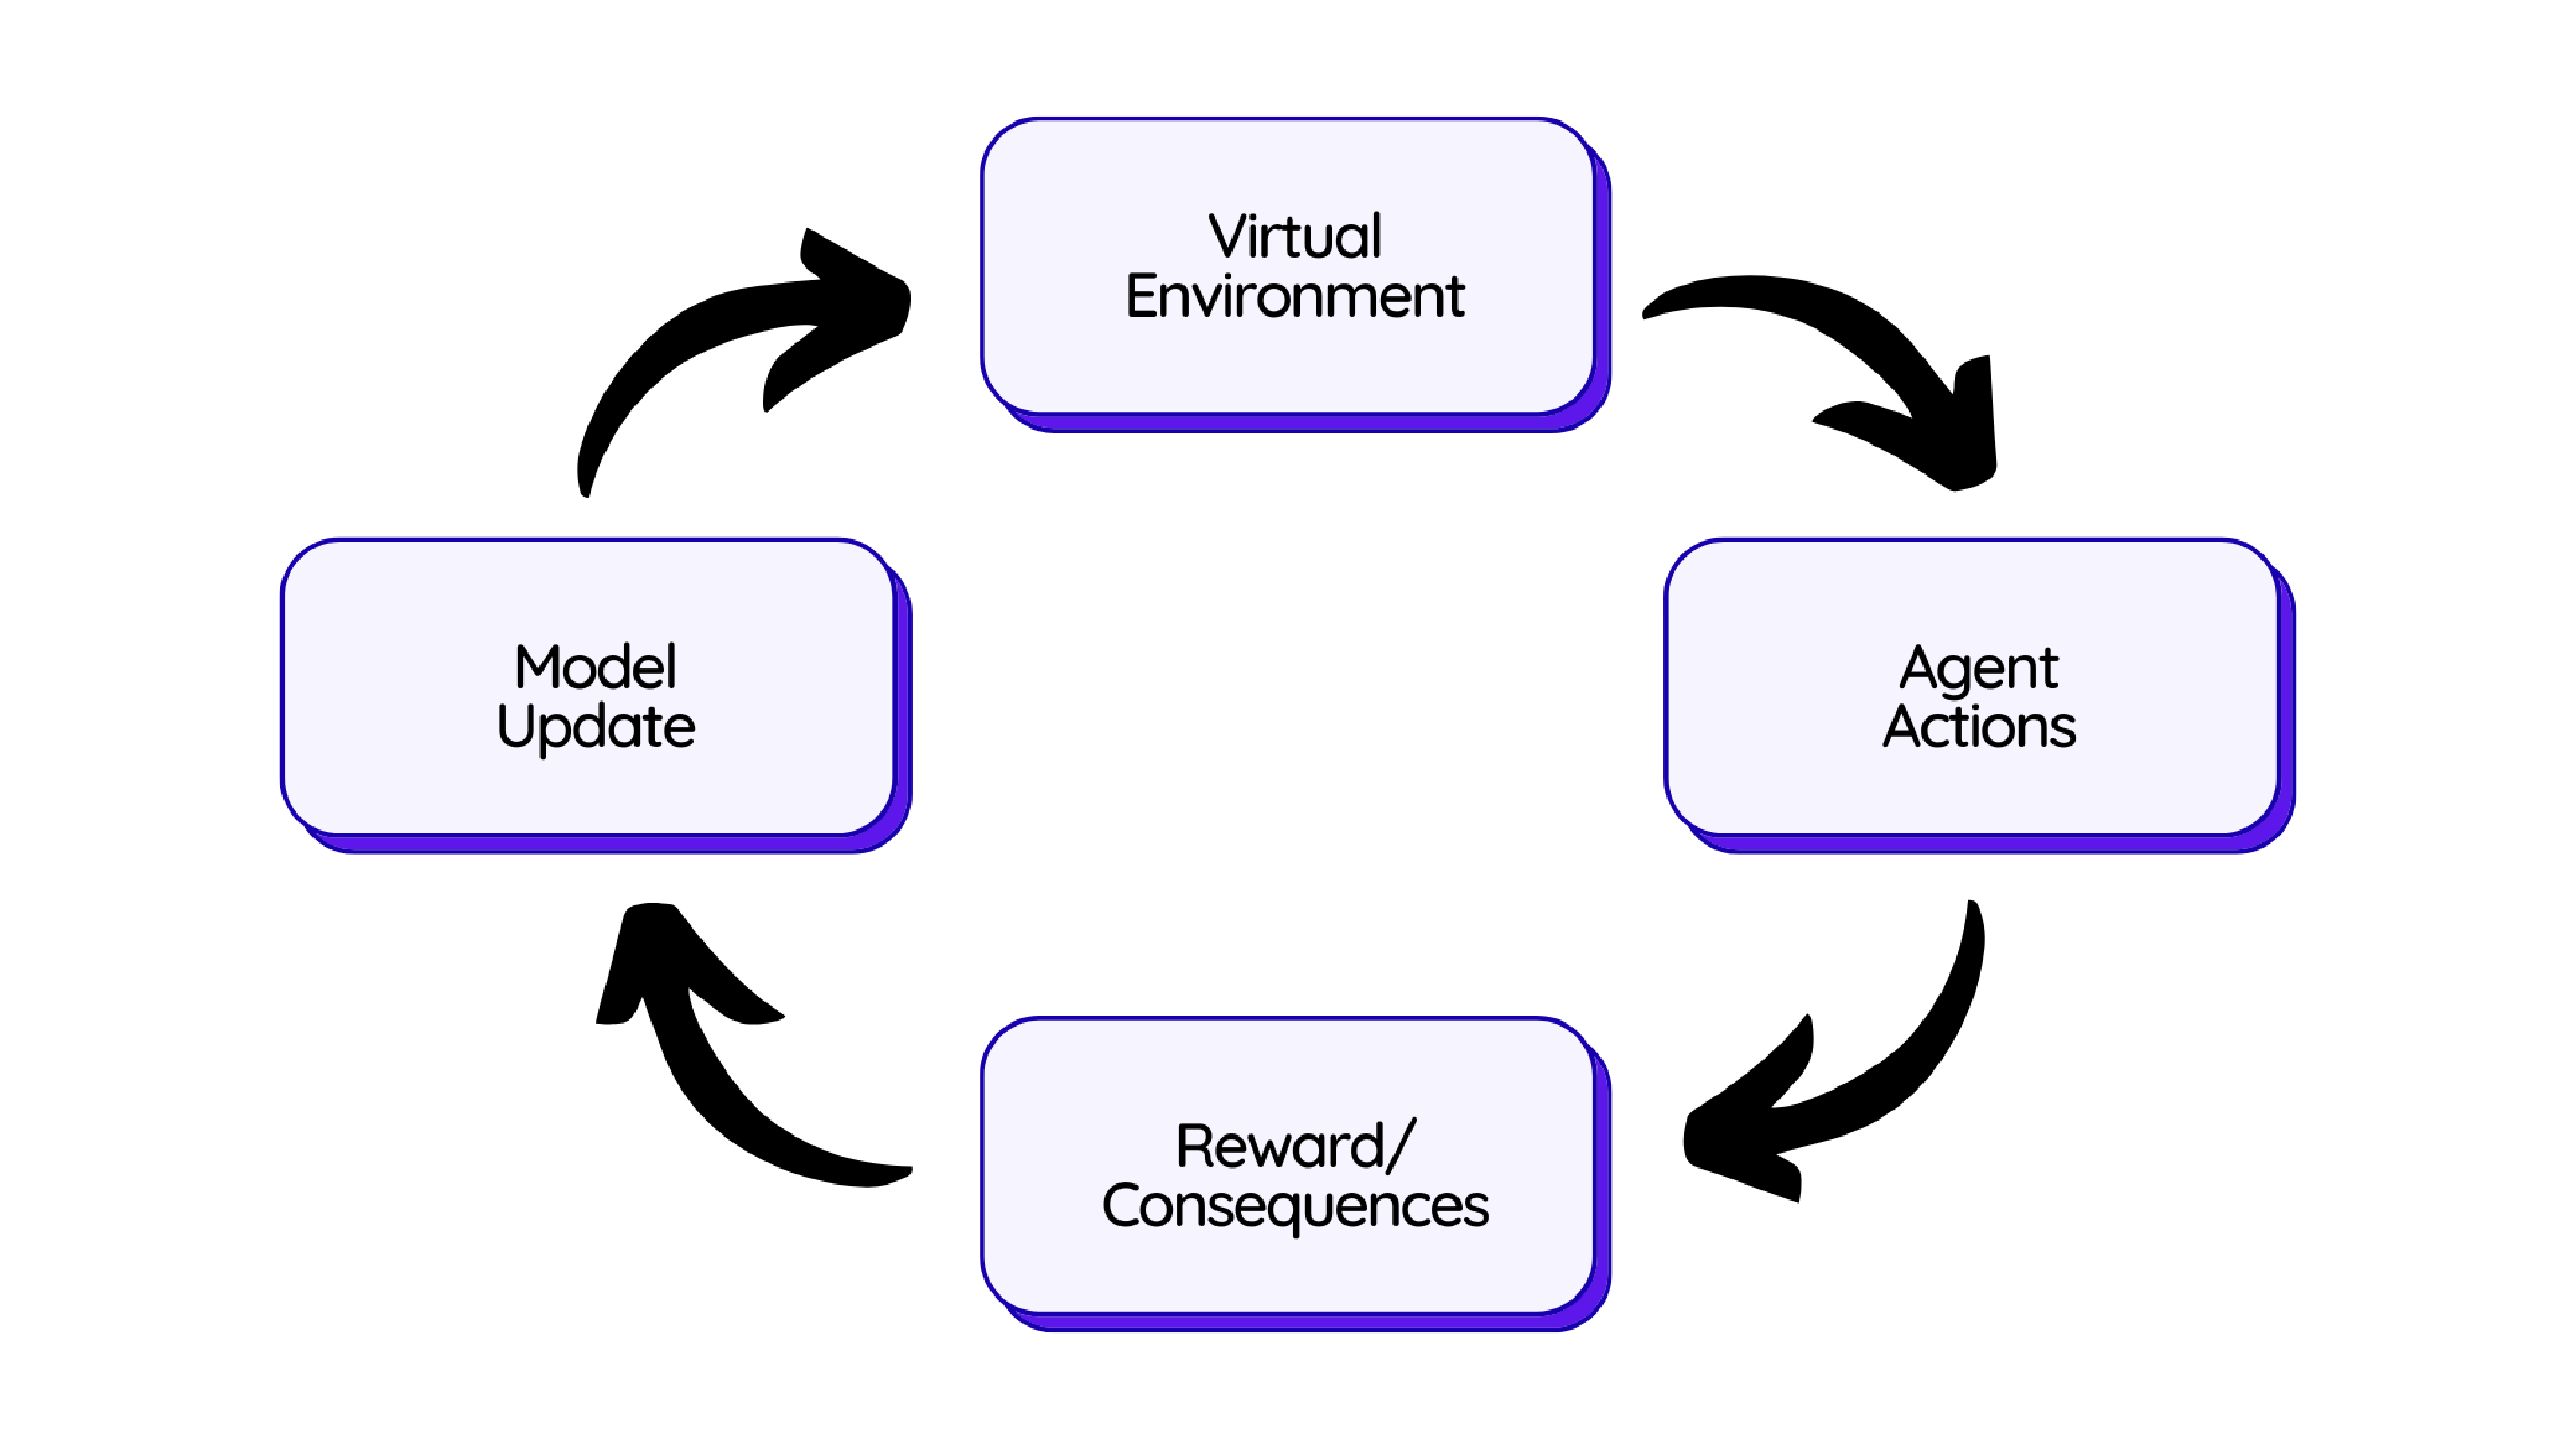
\includegraphics[width=9cm]{images/Pink Sequence Chart (1).pdf}\\
    \caption{Simulation Based Learning}
    \label{fig:sample}
\end{figure}

To address the reality gap, three distinct simulation paradigms have emerged. They are Sim2Real, Digital Twins, and PI (Parallel Intelligence). Let’s look at Sim2Real, which refers to the transfer of knowledge learned from a virtual environment to the real world. It uses techniques like Domain Randomization and Domain Adaptation, where we deliberately vary simulation parameters and try to find the gap between simulated and real data to learn. Digital Twins is a virtual replica of the real world that can be updated in real-time. Parallel Intelligence is a framework where artificial systems (simulated)  and neural systems (real-world) operate in a parallel manner while improving each other.

Synthetic data generation primarily utilizes three approaches: traditional Computer Graphics (CG) for physical precision, Game Engine-based simulations (e.g., CARLA) for creating dynamic, on-demand "corner cases," and Generative AI (GANs) for photorealistic style transfer and scenario creation (Song et al., 2024; Leudet et al., 2018).

The concept of Drivership has been proposed to characterize good driving behaviour (Fraade-Blanar et al., 2024). This framework works on defining an agent's behavior in a simulated environment, it could be both individual and collective expectations of a simulation.

Standard datasets represent structured and western traffic environments but in south asian environments, these datasets fail due to unique class imbalances and chaotic behavior. The presence of Heterogenous Traffic (ex. Non-standard vehicles like Rickshaw, CNGs) propose a unique challenge.



\section{Review of Existing Research}

% \subsection{Importance and Technical Foundations of Simulation \& Synthetic Data}

Complexities are part of training Autonomous Vehicles to achieve fully safe driving on the road. First of all, it is costly and dangerous to run them without being fully prepared. According to the research, billions of miles should be driven by AVs to reach the reliability of human drivers \cite{Hu2023Simulation}. As a consequence, simulation has arrived as a core necessity from a helpful side tool. The problem of collecting massive amounts of training data, usually too expensive to collect, is solved only because of the synthetic data generation process \cite{Song2024Synthetic}. Synthetic datasets allow engineers to increase control over generating high-quality training scenarios. They can accurately adjust lighting, set weather conditions like rain or fog, and create complex traffic scenes that are to be found in real life \cite{Song2024Synthetic}. The importance of this capability is proven because standard testing misses long-tail events–rare but critical safety scenarios that might happen only once every 30,000 miles \cite{Hu2023Simulation, Song2024Synthetic}.\\

Beyond just volume, diversity in training data is crucial to prevent models from failing in new environments, especially to prevent overfitting. Standard datasets generally face difficulties from a “sunny weather bias” or geographic limitations, primarily featuring well structured roads in the USA or Germany \cite{Liu2024Survey, Yu2020BDD100K}. Synthetic data bridges this gap by providing scope to the researchers to generate diverse environmental conditions like heavy monsoon rain, extreme glare, or night-time chaos– ensuring that AV prediction systems work correctly in all situations \cite{Yu2020BDD100K, Goel2024SynDiff}. This diversity is more crucial in the South Asian subcontinent, specifically countries like Bangladesh or India. Since collecting real-world data for every such scenario like indigenous vehicles with unique visual shapes, ignoring strict lane discipline, and various behaviour by the pedestrians is difficult, simulation offers a way to digitally recreate these unstructured environments and indigenous vehicles \cite{Ali2025Microscopic}. This allows AVs to be trained safely for the chaotic reality of cities like Dhaka or Delhi before hitting the physical roads \cite{Pachhapurkar2025ARAI, Hossain2025YOLO}.\\

To make the simulations useful and effective, we must fix the reality gap, which refers to the difference between the virtual world and the real world. Recent studies categorize the methods to do this into three main categories: Sim2Real, Digital Twins, and Parallel Intelligence \cite{Hu2023Simulation}. To maintain the safety of the validation of the sensors and algorithms, these virtual testbeds are crucial. Because of them, researchers get the scope to test how a car handles dangerous failures or extreme driving limits without anyone putting himself at actual risk on public roads \cite{Leudet2018Virtual, Pucher2018Performance}. As we mentioned, we have found that a significant "domain gap" exists in the unstructured and mixed traffic of South Asia. Most current technologies perform well on structured highways by focusing on predictable backgrounds and clearly marked lanes \cite{Varma2018IDD}. However, this gap represents not just a technical obstacle, but a fundamental shift in how a vehicle must perceive and interact with its surroundings and other road users. This gap indicates the lackings in the datasets for traffic and road scenarios for any other countries except the USA and Germany \cite{Liu2024Survey, Yu2020BDD100K}.\\

The first layer of this gap is visual. As established by Baig et al. \cite{Baig2024BadODD} in the BadODD dataset, Bangladeshi roads are filled with unique vehicle classes, such as human-powered rickshaws, CNGs, and modified three-wheelers that are completely missing from the "alphabet of traffic" defined by Western datasets. A similar scenario appears in the IDD dataset \cite{Varma2018IDD}, which highlights that the diversity within vehicle classes on Indian roads is significantly higher. For example, a "truck" in Delhi may look entirely different from a "truck" in Berlin, causing standard detection models to fail.\\

The structural gap is even more profound. Modern autonomous systems are "lane-dependent," relying on geometric rules to plan paths. However, the traffic in South Asia is "area-based." As highlighted in the survey by Min et al. \cite{Li2024Unstructured}, lane markings are load-bearing infrastructure for every major path-planning system in use today, and the moment those markings are treated as optional, where \cite{Ali2025Microscopic} demonstrates through UAV-collected data that lanes are often treated as theoretical suggestions rather than physical boundaries. Instead of following fixed lanes, vehicles, particularly smaller ones like motorcycles and rickshaws, navigate a "continuous drivable surface." This behavior makes standard prediction models ineffective and requires a shift toward "free-space" estimation, where navigation is decided by the physical size of the available gap rather than the legality of the lane.\\

Finally, the gap extends to human behavior. While the PIE dataset \cite{Rasouli2019PIE} successfully uses AI to predict a pedestrian's intent to cross a street in Toronto, these models are blind to the social cues of a South Asian street. In chaotic traffic, "good driving" or Drivership \cite{FraadeBlanar2025Drivership} is defined by mutual understanding and the non-verbal behaviors of pedestrians. Furthermore, as the ARAI India-Specific Scenario report \cite{Pachhapurkar2025ARAI} concludes, unless we recreate specific regional hazards like "cattle on highways" or "wrong-way driving"—in our virtual environments, our autonomous systems will remain technically functional but practically useless in the region.\\

% \subsection{Benchmarks of Success}

Establishing a robust autonomous driving framework needs understanding what “success” is. The literature suggests that we have two benchmarks for it, one is technical verification and another one is social validation. Technical validation ensures sensor reliability and social validation measures the ability of an agent to integrate into human flow of traffic. The baseline of technical performance is well established in structured environments. \cite{Pucher2018Performance} conducted a performance analysis of level 2 autonomous systems using MATLAB route modelling. This confirms that under ideal conditions, such as clear weather and standardized lane marks, there is no notable difference between automated systems and manual human driving. This validatesthe  current generation of sensor hardware like LiDAR, radar, and camera fusion that are mechanically capable of safe navigation. However, \cite{Pucher2018Performance} explicitly noted that the stability is based on “good road infrastructure, which is a critical dependency. It shows that while the hardware is ready, the software reliance on infrastructure will be a point of failure for the unstructured roads of south asian roads. As we move on to the chaotic, “area-based”, heterogeneous traffic of South Asia, technical metrics like “lane deviation” become irrelevant because lanes do not exist. \cite{FraadeBlanar2025Drivership} argue that evaluation must shift from pure safety to "Drivership", the ability of an agent to align with the mutual expectations of other agents in the road. \\

Western models are trained almost exclusively on Normative Expectations (rules, norms, laws). However, South Asian traffic operates heavily on Empirical Expectations (what will likely happen based on experience). Fraade-Blanar et al. conclude that for an AV to be considered "good" in a specific locality, it must satisfy the empirical expectations of that region \cite{FraadeBlanar2025Drivership}. We are not just using synthetic data to teach the car to "see" rickshaws (Technical), but to teach it the "Empirical" behaviors (Social) required to navigate among them without causing severe issues.\\

% \subsection{Implementation}

The final challenge in our methodology is the effective addition of synthetic scenes into modern E2E (End to End) autonomous driving architectures. While synthetic generation allows us to create the “chaotic” paths of heterogeneous traffic, feeding the data into models trained on real world sensors presents a “Domain Gap”.\\

The adaptation of CNN made pattern recognition in computer vision revolutionary, and so has been for autonomous vehicles. Features are automatically learnt from its training data, which makes training a model faster. Implementation of CNN algorithms on parallel computing graphics processing units made automobile driving assistance seem like a possibility of tomorrow. There are levels of autonomous driving vehicles, ranging from level 1 to 5. Up to level 3, human attention to driving is necessary, and driving intervention may be required anytime \cite{Bojarski2016EndToEnd}.\\

Standard E2E models such as UniAd and VAD are sensor-dependent which need raw camera or liDAR inputs to work. In the context of our research, generating photorealistic sensor data for diverse and unique vehicle classes is computationally prohibitive and prone to visual artifacts. Kim et al. \cite{Kim2025SynAD} identifies this bottleneck, understanding that relying solely on real-world sensor data limits the variety of training scenarios, leaving the system vulnerable to rare, unrecorded events. To solve this issue, Kim et al. \cite{Kim2025SynAD} introduces SynAD, a framework designed to enhance real world models using synthetic data without complex sensor rendering. The core innovation is the Map-to-BEV network, which acts as a bridge between simulation and perceptions. In this network, SynAD projects path level scenarios directly into high dimensional BEV (Bird’s Eye View) feature space \cite{Li2022BEVFormer}. This effectively allows the model to learn from spatial logic of the scenario without being distracted by the visual fidelity of the simulation, ans is suited for “Area-Based” navigation challenges like the domain gap we found in our literature review.\\

 
\section{Summary of Key Findings}

\begin{table}[h!]
    \centering
    \begin{tabular}{|p{3.5cm}|p{4cm}|p{3.9cm}|p{1.9cm}|}
    \hline
    \textbf{Paper / Author} & \textbf{Methodologies} & \textbf{Findings}& \textbf{Year}\\
    \hline
    End to end learning for self-driving cars (Bojarski et al.) & 
    Trained a CNN model to map raw camera data directly to steering wheel. & 
    CNN learned entire task of lane and road following without manual decomposition into road or lane marking detection, semantic abstraction, path planning, and control. & 
    2016 \\
    \hline
    Virtual environment for training autonomous vehicles (Leudet et al.) & 
    Virtual simulation environments (Unity/Game engines) mimicking real sensors (Lidar/Camera). & 
    Confirmed simulation as a dual-purpose tool for safely testing algorithms in dangerous scenarios and generating training data. & 
    2018 \\
    \hline
    Performance analysis of vehicle-specific methods... (Pucher et al.) & 
    Comparison of manual vs. semi-autonomous driving using MATLAB/Simulink and vehicle dynamics sensors. & 
    AVs perform comparably to humans in good infrastructure; sensor reliability drops significantly in adverse weather/road conditions. & 
    2018 \\
    \hline
    IDD: A dataset for exploring problems... (Varma et al.) & 
    IDD (Indian Driving Dataset); 4-level label hierarchy for unstructured traffic. & 
    Western models (e.g., trained on Cityscapes) fail in India; identified unique classes like "drivable area" vs. road. & 
    2018 \\
    \hline
    PIE: A large-scale dataset... (Rasouli et al.) & 
    PIE Dataset; RNN/LSTM models for pedestrian intention prediction. & 
    Context (traffic lights, looking at car) is crucial; intention prediction requires temporal analysis, not just static pose. & 
    2019 \\
    \hline
    BDD100K: A diverse driving dataset... (Yu et al.) & 
    BDD100K (100k videos); Heterogeneous Multitask Learning. & 
    Validated that high diversity in weather, time, and location is essential to prevent model overfitting; enables multi-task learning. & 
    2020 \\
    \hline
    \end{tabular}
\end{table}
\begin{table}[h!]
    \centering
    \begin{tabular}{|p{3.5cm}|p{4cm}|p{3.9cm}|p{1.9cm}|}
    \hline
    \textbf{Paper / Author} & \textbf{Methodologies} & \textbf{Findings}& \textbf{Year}\\
    \hline
    Bevformer: Learning bird’s-eye-view representation... (Li et al.) & 
    BEVFormer (Spatiotemporal Transformers); nuScenes. & 
    Achieved state-of-the-art 3D detection and velocity estimation by transforming multi-camera inputs into a unified Bird's-Eye-View. & 
    2022 \\
    \hline
    How simulation helps autonomous driving... (Hu et al.) & 
    Survey of Sim2Real, Digital Twins, and Parallel Intelligence. & 
    Simulation is evolving from simple testing to closed-loop "Parallel Intelligence" systems to bridge the Reality Gap. & 
    2023 \\
    \hline
    BadODD: Bangladeshi autonomous driving object detection dataset (Baig et al.) & 
    BadODD dataset; Object detection for regional vehicles. & 
    Established a dataset containing unique Bangladeshi vehicles (Rickshaws, CNGs) absent in global datasets. & 
    2024 \\
    \hline
    Improving end-to-end autonomous driving... (Goel \& Narasimhan) & 
    SynDiff-AD (Latent Diffusion Models); Synthetic variations of standard sets. & 
    Improved segmentation (Mask2Former) by +1.4 mIoU and planning by 20\% by synthesizing rare weather conditions (rain/fog). & 
    2024 \\
    \hline
    Autonomous driving in unstructured environments... (Li et al.) & 
    Survey of path planning in unstructured traffic. & 
    Highlighted that "lane-based" planning fails in unstructured roads; proposed shift to "area-based" or "free-space" navigation. & 
    2024 \\
    \hline
    A survey on autonomous driving datasets... (Liu et al.) & 
    Statistical analysis of 265 datasets; "Impact Score". & 
    Identified severe geographic bias (45\% US/Germany); confirmed lack of "long-tail" safety scenarios in naturalistic data. & 
    2024 \\
    \hline
    Synthetic datasets for autonomous driving: A survey (Song et al.) & 
    Survey of synthetic generation techniques (Game engines vs. Generative AI). & 
    Synthetic data acts as a "data factory" for corner cases where real-world data collection is too expensive or dangerous. & 
    2024 \\
    \hline
    \end{tabular}
\end{table}
\begin{table}[h!]
    \centering
    \begin{tabular}{|p{3.5cm}|p{4cm}|p{3.9cm}|p{1.9cm}|}
    \hline
    \textbf{Paper / Author} & \textbf{Methodologies} & \textbf{Findings}& \textbf{Year}\\
    \hline
    Microscopic vehicle trajectory datasets... (Ali et al.) & 
    UAV (Drone) video collection in India; Trajectory data. & 
    Vehicles in mixed traffic ignore lanes and utilize lateral space ("creeping"); defined non-linear flow dynamics of heterogeneous traffic. & 
    2025 \\
    \hline
    Being good (at driving): Characterizing behavioral expectations... (Fraade-Blanar et al.) & 
    Conceptual framework (Drivership). & 
    Differentiated between Normative (legal) and Empirical (social) expectations; AVs must learn social behaviors to be accepted. & 
    2025 \\
    \hline
    Evaluating YOLO architectures... (Hossain et al.) & 
    YOLO v8, v9, v10 evaluation on Bangladesh traffic footage. & 
    Generic YOLO models fail on indigenous vehicles (Leguna, Nosimon); requires architecture-specific tuning for local classes. & 
    2025 \\
    \hline
    SynAD: Enhancing real-world end-to-end... (Kim et al.) & 
    SynAD framework; Map-to-BEV network. & 
    Enhances real-world models by projecting synthetic path-level scenarios into BEV space, avoiding visual domain gap artifacts. & 
    2025 \\
    \hline
    Developing India-specific virtual scenarios... (Pachhapurkar) & 
    Real-to-Sim workflow; IPG CarMaker; Scenario Builder. & 
    Created a library of validated "cut-in" and "cattle on road" scenarios specifically for testing ADAS on Indian roads. & 
    2025 \\
    \hline
    \end{tabular}
    \caption{Key Findings and Summary}
    \label{tab:placeholder}
\end{table}

